% =========================================================================
%  pycorrect vs MCAMS -- comparison report
%  Attenuation (Paalman & Pings) and multiple scattering (Blech & Averbach)
%  computed analytically (pycorrect / CORRECT 2.24) and by Monte Carlo (MCAMS)
%  Compile with:  latexmk -pdf main.tex   (or pdflatex main.tex, three times)
%  Figures: python ../compare_pycorrect_mcams.py ; python ../example_d4_with_mcams.py
% =========================================================================
\documentclass[11pt,a4paper]{report}
% ======================================================================
% preamble.tex - packages, macros and styles of the MCAMS manual
% (same style as the MCAMS and pycorrect manuals)
% ======================================================================
\usepackage[T1]{fontenc}
\usepackage[utf8]{inputenc}
\usepackage{mathpazo}
\renewcommand{\ttdefault}{txtt}   % txfonts typewriter: narrower than Courier
\usepackage{microtype}
% no ligatures in typewriter text: "--fullness" must not become an en-dash
\DisableLigatures[-]{encoding = T1, family = tt*}
\usepackage[english]{babel}
\usepackage[a4paper,margin=2.5cm,headheight=14pt]{geometry}
\usepackage{amsmath,amssymb}
\usepackage{graphicx}
\usepackage{booktabs,tabularx,longtable,array}
\usepackage{xcolor}
\usepackage{listings}
\usepackage[most]{tcolorbox}
\usepackage{enumitem}
\usepackage{fancyhdr}
\usepackage{titlesec}
\usepackage{caption}
\usepackage{float}
\usepackage{tikz}
\usetikzlibrary{arrows.meta,positioning,shapes.geometric}
\usepackage[colorlinks=true,linkcolor=accent,urlcolor=accent,citecolor=accent]{hyperref}

\graphicspath{{../figures/}}
\setcounter{tocdepth}{1}
\emergencystretch=2em

% ---------------------------------------------------------------- colours
\definecolor{accent}{HTML}{2A78D6}
\definecolor{accent2}{HTML}{EB6834}
\definecolor{accent3}{HTML}{1BAF7A}
\definecolor{ink2}{HTML}{52514E}
\definecolor{codebg}{HTML}{F6F6F4}
\definecolor{outbg}{HTML}{EEF4FC}
\definecolor{noteback}{HTML}{EEF4FC}
\definecolor{warnback}{HTML}{FDF0EA}

% ---------------------------------------------------------------- headings
\titleformat{\chapter}[display]{\normalfont\bfseries\color{accent}}
  {\large\scshape \chaptertitlename\ \thechapter}{4pt}{\Huge}
\titlespacing*{\chapter}{0pt}{-20pt}{24pt}
\titleformat{\section}{\normalfont\Large\bfseries\color{accent}}{\thesection}{0.8em}{}
\titleformat{\subsection}{\normalfont\large\bfseries}{\thesubsection}{0.8em}{}

\pagestyle{fancy}
\fancyhf{}
\fancyhead[L]{\small\color{ink2}\textsc{pycorrect} vs \textsc{mcams}}
\fancyhead[R]{\small\color{ink2}\nouppercase{\leftmark}}
\fancyfoot[C]{\small\thepage}
\renewcommand{\headrulewidth}{0.4pt}

% ---------------------------------------------------------------- code
% Python code, program output and shell commands. The chapters use
%   \begin{lstlisting} ... \end{lstlisting}            (Python, default)
%   \begin{lstlisting}[style=shell] ... \end{lstlisting}
%   \pyexample{name}  (examples/name.py followed by examples/output/name.txt)
\lstdefinestyle{base}{
  basicstyle=\ttfamily\small, backgroundcolor=\color{codebg},
  frame=single, rulecolor=\color{codebg}, framesep=4pt, xleftmargin=4pt,
  xrightmargin=4pt, breaklines=true, columns=fullflexible, keepspaces=true,
  showstringspaces=false, aboveskip=8pt, belowskip=8pt,
  commentstyle=\color{ink2}\itshape, keywordstyle=\color{accent}\bfseries,
  stringstyle=\color{accent2}, upquote=true}
\lstdefinestyle{pycode}{style=base, language=Python}
\lstdefinestyle{shell}{style=base, language={}}
\lstdefinestyle{output}{style=base, language={}, basicstyle=\ttfamily\scriptsize,
  backgroundcolor=\color{outbg}, rulecolor=\color{outbg}, aboveskip=0pt}
\lstset{style=pycode}

\newcommand{\pyexample}[1]{%
  \lstinputlisting[style=pycode]{examples/#1.py}%
  \lstinputlisting[style=output]{examples/output/#1.txt}}

% \code{...}: typewriter text for names, calls and short pieces of code.
% Spaces, underscores and other special characters are allowed inside; braces
% must be balanced. Do not use it in titles or captions (use \texttt there).
\newcommand{\code}[1]{\texttt{\detokenize{#1}}}
\newcommand{\file}[1]{\texttt{#1}}

% ---------------------------------------------------------------- boxes
\newtcolorbox{note}[1][Note]{colback=noteback,colframe=accent,boxrule=0pt,
  leftrule=3pt,arc=0pt,fonttitle=\bfseries,coltitle=accent,colbacktitle=noteback,
  title=#1,attach title to upper={\ \ },before skip=8pt,after skip=8pt}
\newtcolorbox{warn}[1][Caution]{colback=warnback,colframe=accent2,boxrule=0pt,
  leftrule=3pt,arc=0pt,fonttitle=\bfseries,coltitle=accent2,colbacktitle=warnback,
  title=#1,attach title to upper={\ \ },before skip=8pt,after skip=8pt}
\newtcolorbox{fnbox}[1]{colback=white,colframe=accent,boxrule=0.6pt,arc=2pt,
  fonttitle=\ttfamily\bfseries,coltitle=white,title={#1},before skip=10pt,after skip=6pt}

\setlist{itemsep=2pt,topsep=4pt}
\captionsetup{font=small,labelfont={bf,color=accent}}
\setlength{\parindent}{0pt}
\setlength{\parskip}{5pt}

% ---------------------------------------------------------------- macros
\newcommand{\mcams}{\textsc{mcams}}
\newcommand{\twotheta}{2\theta}
\newcommand{\mumm}{\mu\ (\mathrm{mm}^{-1})}
\newcommand{\deriv}[1]{\mathrm{d}#1}
\DeclareMathOperator{\e}{e}
\newcommand{\pyc}{\textsc{pycorrect}}
\newcommand{\cor}{\textsc{correct}}
\setcounter{tocdepth}{1}


\begin{document}

% ---------------------------------------------------------------- title
\begin{titlepage}
\thispagestyle{empty}
\vspace*{2.5cm}
{\color{accent}\rule{\linewidth}{2pt}}\par\vspace{0.6cm}
{\fontsize{34}{40}\selectfont\bfseries\pyc\ \normalfont vs\ \bfseries\mcams}\par\vspace{0.4cm}
{\LARGE Attenuation and multiple scattering:\\[2pt] analytical corrections against Monte Carlo}\par\vspace{0.3cm}
{\Large\color{ink2} Paalman \& Pings factors and Blech \& Averbach multiple scattering
of \cor\ 2.24 compared with particle trajectories}\par
\vspace{0.6cm}{\color{accent}\rule{\linewidth}{2pt}}\par
\vspace{1.5cm}
{\Large Comparison report}\par
\vfill
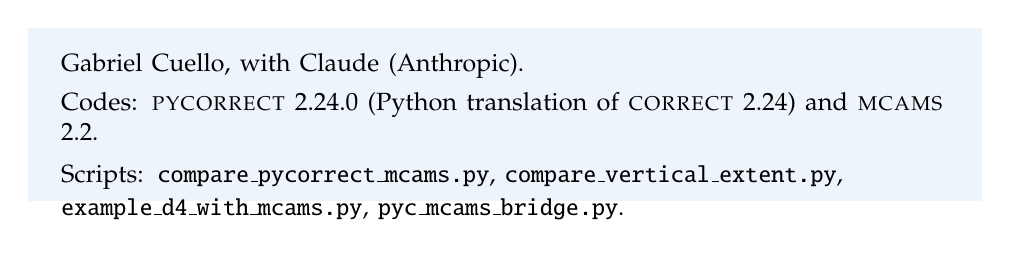
\begin{tikzpicture}
  \fill[noteback] (0,0) rectangle (\linewidth,2.2);
  \node[anchor=north west,text width=0.95\linewidth,align=left] at (0.3,2.0) {
  \small Gabriel Cuello, with Claude (Anthropic).\\[3pt]
  Codes: \pyc\ 2.24.0 (Python translation of \cor\ 2.24) and \mcams\ 2.2.\\[3pt]
  Scripts: \file{compare\_pycorrect\_mcams.py}, \file{compare\_vertical\_extent.py},
  \file{example\_d4\_with\_mcams.py}, \file{pyc\_mcams\_bridge.py}.};
\end{tikzpicture}
\vspace{1cm}
{\small\color{ink2}\today}
\end{titlepage}

\pagenumbering{roman}
\tableofcontents
\clearpage
\pagenumbering{arabic}

% =========================================================================
\chapter{Introduction and summary}
% =========================================================================

\pyc\ (the Python version of \cor\ 2.24) corrects neutron diffraction data with
analytical models: the \textbf{Paalman \& Pings} attenuation factors, computed by
numerical integration over the cross-section of a cylindrical sample, container
and furnace, and the \textbf{Blech \& Averbach} multiple-scattering correction,
taken from a table of the double-to-single scattering ratio and extended to
higher orders by an empirical series.

\mcams\ (Monte Carlo Attenuation and Multiple Scattering) follows individual
neutron trajectories through the same layered cylinder, with the same beam and
detector geometry. It contains attenuation and multiple scattering but no
inelasticity (Placzek) and no vanadium normalisation. The comparison is therefore
restricted to these two effects.

The aims of this report are
\begin{enumerate}
  \item to compute with \mcams\ exactly the quantities that \pyc\ uses, and to
        compare them for representative geometries;
  \item to establish which approximations of \cor\ matter, and by how much;
  \item to explain how to use \mcams\ to do what \pyc\ does;
  \item to test the treatment of partially filled containers, using the layers
        with their own bottom and height of \mcams~2.2 (Chapter~\ref{chap:vertical}).
\end{enumerate}

\section*{Main results}

\begin{note}[Attenuation]
For a beam wider than the sample the Paalman \& Pings factors of \pyc\ and
\mcams\ agree within the Monte Carlo error, 0.1--0.5\% (sample alone, sample in
a can, can alone). Two approximations of \cor\ show up:
\begin{itemize}
  \item \textbf{Narrow beam} (0.2~cm beam on a 0.6~cm sample): \pyc\ overestimates
        $A_{s,sc}$ by 1.0--1.2\% at all angles. A third, independent calculation
        agrees with \mcams\ to 0.03\%.
  \item \textbf{Furnace}: \cor\ computes the furnace factors at 0, 90 and
        180$^\circ$ only and joins them with a parabola. The true $A_{h,sch}$ has
        dips near 30$^\circ$ and 150$^\circ$, where the scattered beam from the
        furnace wall crosses the sample. The parabola misses them by up to 9\%.
        $A_{h,h}$ and $A_{h,ch}$ are off by about 1\%. At 0, 90 and 180$^\circ$
        \pyc\ is exact.
\end{itemize}
\end{note}

\begin{note}[Multiple scattering]
\begin{itemize}
  \item The \textbf{Blech \& Averbach table} of the double-scattering ratio
        $\delta_2$ is confirmed by \mcams: mostly within 1\% for $\mu R \leq 1$
        (up to 2\% for the smallest values) and within 2.5\% up to $\mu R = 2$,
        for $R/H$ between 0.1 and 1.
  \item The \textbf{empirical series} of \cor\ for the higher orders,
        $\delta = d + 0.694 d^2 + 0.370 d^3 + \dots$, underestimates them
        strongly. In the simulations each order is about $(1.03$--$1.2)\,d$
        times the previous one, not $0.694\,d$. For the Ni example ($\mu R =
        0.54$, $\sigma_s/\sigma_t = 0.94$) \pyc\ gives $\delta = 0.486$ against
        0.58--0.63 from \mcams; for a pure scatterer with $\mu R = 1$, 0.81
        against 1.31.
  \item $\delta$ depends on angle (about $\pm 3.5\%$ for the Ni sample), and it
        grows when the sample is taller than the beam (+7.5\% for a sample
        3.3 times taller). Both effects are ignored by \cor.
\end{itemize}
\end{note}

\begin{note}[Partially filled samples and flat plates (Chapter~\ref{chap:vertical})]
\begin{itemize}
  \item The \textbf{fullness} step of \cor\ is exact for single scattering,
        wherever the powder sits in the beam, if the can covers the whole beam
        and the beam is uniform. It is wrong by $-1.1\%$ when the can bottom is
        inside the beam (a fixed recipe is given), and by $-33\%$ for a Gaussian
        beam profile unless the flux fraction is used.
  \item The multiple-scattering correction of \cor\ ignores the fullness.
  \item Two errors were found in the Fortran \code{PLATE} (flat-plate factors):
        $A_{c,sc}$ in reflection geometry (0.82 instead of 0.61 in the test
        cell) and $A_{c,c}$ doubled at $2\theta = 0$. They are corrected in
        \pyc\ (\code{faithful=False}).
\end{itemize}
\end{note}

% =========================================================================
\chapter{The two approaches}
\label{chap:methods}
% =========================================================================

\section{Common geometry and units}

Both programs describe a two-axis instrument: the beam travels horizontally
($+z$ in \mcams), the cylinders are vertical and centred on the axis of the
detector circle, and the detector moves in the horizontal plane. \pyc\ works in
cm and cm$^{-1}$, \mcams\ in mm and mm$^{-1}$. All the inputs below are given in
\pyc\ units; the bridge module converts them (Table~\ref{tab:map}).

\begin{table}[H]
\centering\small
\begin{tabularx}{\linewidth}{@{}>{\raggedright\arraybackslash}p{4.6cm}>{\raggedright\arraybackslash}X@{}}
\toprule
\pyc\ (\code{atcors}, \code{mscat}) & \mcams\ \\
\midrule
sample radius $R_1$ (cm) & innermost layer, thickness = \textbf{diameter} $20R_1$ (mm) \\
container outer radius $R_2$ & annular layer, radial thickness $10(R_2-R_1)$ \\
furnace radii $R_3, R_4$ & a layer with $\mu=0$ (gap, $10(R_3-R_2)$) and a layer of thickness $10(R_4-R_3)$ \\
total $\mu$ (cm$^{-1}$) & \code{mu} $=\mu/10$ (mm$^{-1}$) \\
$\mu_s/\mu_t$ (used in \code{mscat}) & \code{scatter_fraction} \\
beam width (cm) & \code{beam_width} (mm) \\
beam height $H$ (cm) & \code{beam_height} (mm); sample height chosen separately \\
\bottomrule
\end{tabularx}
\caption{Correspondence of the inputs. $\mu = n(\sigma_s + \sigma_a\lambda/1.798)$
with $n$ in \AA$^{-3}$ and $\sigma$ in barn gives $\mu$ in cm$^{-1}$.}
\label{tab:map}
\end{table}

\section{Attenuation factors}

\paragraph{\pyc.} For a scattering body $k$ of cross-section $S_k$ (the part inside
the beam if the beam is narrower than the body),
\begin{equation}
  A_k(2\theta) = \frac{1}{S_k}\int_{S_k} \e^{-\sum_m \mu_m\,[l_m^{\text{in}}(\mathbf r)+l_m^{\text{out}}(\mathbf r,2\theta)]}\,dS ,
  \label{eq:pp}
\end{equation}
integrated with 9$\times$9 Gauss--Legendre points in polar coordinates
(\code{atcors}). The furnace factors are computed at $2\theta = 0, 90, 180^\circ$
and interpolated with a parabola.

\paragraph{\mcams.} The function \code{transmission_by_last_layer} draws the first
interaction point of each incident neutron with the Beer--Lambert law. The
attenuation on the way \emph{in} is therefore already in the distribution of the
points. At every scattering event in layer $k$ it records the attenuation on the
way \emph{out}, $\e^{-\sum_m\mu_m l_m^{\text{out}}}$, for every detector angle.
Summed over the first scatterings and divided by the number of incident
neutrons $N$, this gives, for a beam of width $W$ lower than the sample,
\begin{equation}
  \frac{\Sigma_k^{(1)}(2\theta)}{N} = \frac{f_k\mu_k}{W}
  \int_{S_k}\e^{-\sum_m \mu_m(l^{\text{in}}_m+l^{\text{out}}_m)}\,dS ,
\end{equation}
where $f_k$ is the scatter fraction. Dividing by the value it would have without
attenuation, $f_k\mu_k S_k/W$, gives exactly equation~(\ref{eq:pp}):
\begin{equation}
  \boxed{A_k(2\theta) = \frac{\Sigma_k^{(1)}(2\theta)/N}{f_k\,\mu_k\,S_k/W}}
  \label{eq:mcA}
\end{equation}
$S_k$ is computed with the function \code{area(r, d)} of \pyc\ (area of a circle
inside a band of half-width $d$). The factors $A_{c,ch}$, $A_{h,ch}$ and
$A_{h,h}$ refer to the empty container or the furnace alone. They are obtained
by running \mcams\ again with $\mu=0$ in the inner bodies: the layers are kept,
but they neither attenuate nor scatter.

\section{Multiple scattering}

\paragraph{\pyc.} \code{mscat(R, H, mu_t, mu_s)} interpolates
$\delta_2(\mu R, R/H)$, the ratio of doubly to singly scattered intensity for an
isotropic scatterer (Blech \& Averbach~\cite{ba}). It computes
$d = \delta_2\,\mu_s/\mu_t$ and returns
\begin{equation}
  \delta = d + 0.693957\,d^2 + 0.370110\,d^3 + 0.160525\,d^4 + 0.058706\,d^5 ,
  \label{eq:series}
\end{equation}
a single number for all angles. For a sample in a can \cor\ uses an effective
cylinder of radius $R_2$ with volume-averaged coefficients.

\paragraph{\mcams.} The same random walk is followed to all orders (isotropic
scattering, absorption with probability $1-f_k$). Let $\Sigma^{(n)}(2\theta)$ be
the sum, over the $n$-th scattering events, of the attenuation towards the
detector. Then
\begin{equation}
  \delta_2^{\text{MC}} = \frac{\Sigma^{(2)}}{\Sigma^{(1)}}, \qquad
  \delta^{\text{MC}} = \frac{\sum_{n\geq 2}\Sigma^{(n)}}{\Sigma^{(1)}} ,
\end{equation}
both functions of $2\theta$.

The \mcams\ function \code{transmission_by_last_layer} gives
$\delta^{\text{MC}}$ directly, as the ratio of its ``multiple'' and ``single''
sums. The
order-by-order sums need a small loop with the same \mcams\ building blocks
(\code{mc_scattering_orders} in \file{pyc\_mcams\_bridge.py}). Like Blech \&
Averbach, $\delta_2$ already contains $\mu_s/\mu_t$: in the simulation a second
event is a scattering only with probability $f$. It is therefore compared with
$f\,\delta_2^{\text{table}}$.

\begin{note}[Same definition]
In both programs $\delta$ is the ratio of the intensities that reach the
detector (each attenuated on its way out), which is what \cor\ subtracts:
$d\sigma/d\Omega = I_s/I_v\cdots - \delta\,\sigma_s/4\pi$.
\end{note}

% =========================================================================
\chapter{Set-up of the comparison}
% =========================================================================

\section{Materials and geometries}

The example of the \pyc\ manual is used: a nickel sample in a vanadium can at
$\lambda = 0.4985$~\AA.

\begin{center}\small
\begin{tabular}{@{}lccccc@{}}
\toprule
 & $n$ (\AA$^{-3}$) & $\sigma_s$ (b) & $\sigma_a$ (b) & $\mu_t$ (cm$^{-1}$) & $\mu_s/\mu_t$ \\
\midrule
Ni & 0.0913 & 18.5 & 4.49 & 1.8027 & 0.9370 \\
V  & 0.0722 & 4.95 & 5.08 & 0.4591 & 0.7785 \\
\bottomrule
\end{tabular}
\end{center}

\begin{center}\small
\begin{tabularx}{\linewidth}{@{}l>{\raggedright\arraybackslash}X@{}}
\toprule
Case & Geometry \\
\midrule
A1 & Ni rod, $R_1 = 0.30$~cm, beam 1.5~cm wide (wider than the sample) \\
A2 & Ni in a V can, $R_1 = 0.30$, $R_2 = 0.32$~cm, beam 1.5~cm \\
A3 & as A2 with a 0.2~cm beam (narrower than the sample) \\
A4 & as A2 inside a V furnace, $R_3 = 1.00$, $R_4 = 1.04$~cm, beam 1.5~cm \\
B1 & pure scatterer ($f = 1$), $R = 0.30$~cm, $\mu R = 0.1$--2, $R/H = 0.1, 0.25, 0.5, 1$ \\
B2 & as B1 with $f = 0.5$, $R/H = 0.1$ \\
B3 & Ni rod and Ni in V can, $H = 3$~cm, $\delta$ versus $2\theta$ \\
B4 & Ni rod, beam height 3~cm, sample height 3 to 10~cm \\
D4 & the complete D4 example of the \pyc\ manual run with both programs \\
\bottomrule
\end{tabularx}
\end{center}

For the attenuation cases (A) the sample is 5~cm tall and the beam 2~cm high.
Single scattering into a horizontal detector then never reaches the top or
bottom faces: the geometry is the two-dimensional one of Paalman \& Pings. For
the multiple-scattering cases (B1--B3) the sample height equals the beam height
$H$, as assumed by Blech \& Averbach and by \cor, which uses the beam height.

\section{Statistics}

Every Monte Carlo number is the mean of independent runs with different seeds
(10 runs of $4\times10^5$ neutrons for A, 8 runs of $6\times10^4$ to $10^5$ for
B). The error bars are the standard error of the mean. In each run the same
neutrons are used for all the angles, so the errors at different angles are
correlated: a whole curve can be shifted by about one error bar. The full
comparison takes about 4 minutes on a laptop (\code{--quick}: 20 seconds).

\section{Independent check}

Where the two programs disagree, a third calculation was made (part C of the
script). The scattering point is sampled uniformly over the body (inside the
beam), and the exact in and out chord lengths in every circle give the
attenuation. This method shares no code with either program.

% =========================================================================
\chapter{Attenuation: results}
% =========================================================================

\section{Beam wider than the sample (A1, A2)}

\begin{figure}[H]
  \centering
  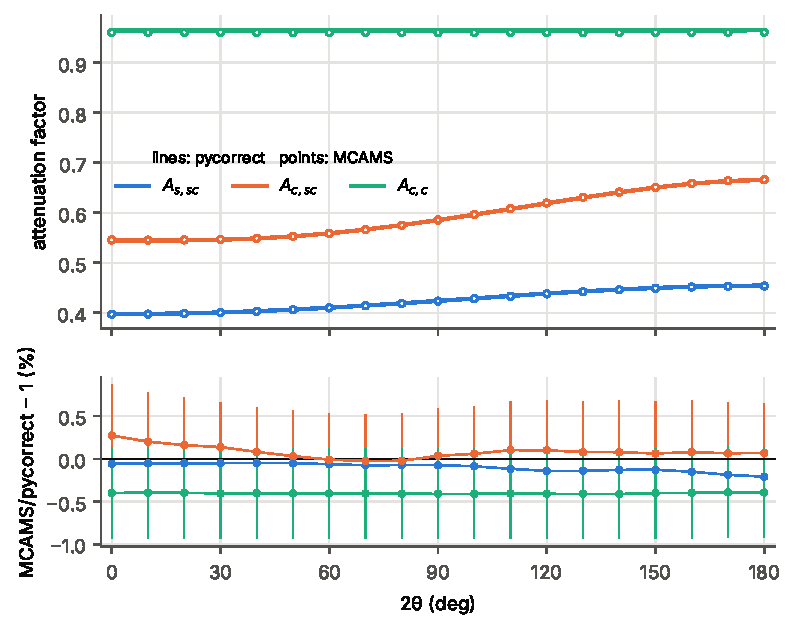
\includegraphics[width=0.82\linewidth]{A2_sample_in_can.pdf}
  \caption{Ni in a V can, beam wider than the can (case A2). Upper panel: lines
  \pyc, open points \mcams. Lower panel: relative difference.}
  \label{fig:A2}
\end{figure}

\begin{center}\small
\begin{tabular}{@{}llccc@{}}
\toprule
Case & factor & max $|\text{MC}/\text{pyc}-1|$ & mean difference & MC error \\
\midrule
A1 & $A_{s,s}$  & 0.23\% & $-0.12$\% & 0.11\% \\
A2 & $A_{s,sc}$ & 0.21\% & $-0.10$\% & 0.11\% \\
A2 & $A_{c,sc}$ & 0.27\% & $+0.08$\% & 0.57\% \\
A2 & $A_{c,c}$  & 0.41\% & $-0.40$\% & 0.53\% \\
\bottomrule
\end{tabular}
\end{center}

The agreement is within the statistical error (Figure~\ref{fig:A2}). The
quadrature of \cor\ is very accurate when the beam covers the whole sample.

\section{Beam narrower than the sample (A3)}

\begin{figure}[H]
  \centering
  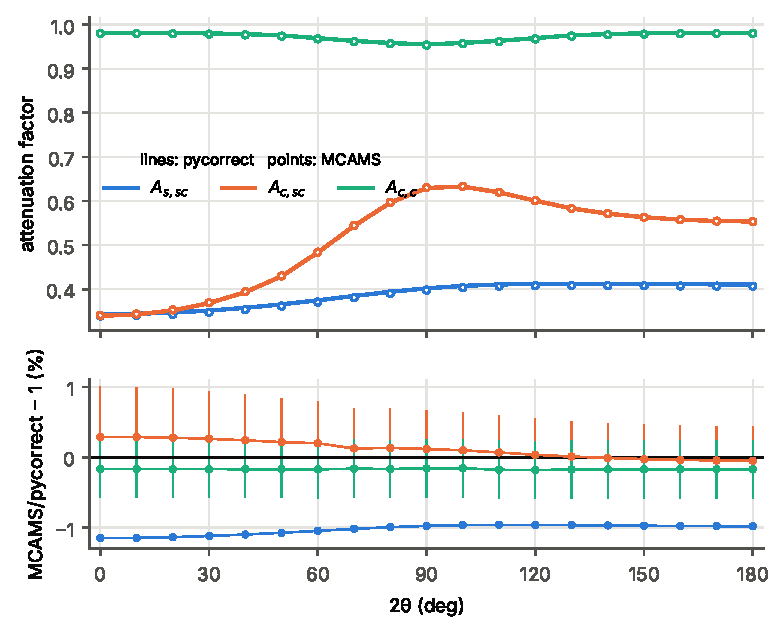
\includegraphics[width=0.82\linewidth]{A3_narrow_beam.pdf}
  \caption{Same sample with a 0.2~cm beam (case A3).}
  \label{fig:A3}
\end{figure}

$A_{s,sc}$ from \pyc\ is 1.0--1.2\% higher than from \mcams\ at all angles, far
beyond the error (0.03\%). The independent calculation sides with \mcams:

\begin{center}\small
\begin{tabular}{@{}lcccc@{}}
\toprule
$2\theta$ & \pyc & \mcams & error & direct sampling \\
\midrule
0$^\circ$   & 0.34351 & 0.33955 & 0.00014 & 0.33957 \\
90$^\circ$  & 0.40201 & 0.39808 & 0.00013 & 0.39817 \\
180$^\circ$ & 0.41098 & 0.40694 & 0.00013 & 0.40706 \\
\bottomrule
\end{tabular}
\end{center}

When the beam is narrower than the body, \cor\ cuts the angular integration limits
at the beam edges. This produces kinks that a single 9-point Gauss panel does not
resolve well; the error depends on the geometry (0.4\% was found in the
self-tests of \pyc\ for another case). In this case the container factors
agree within their (larger) statistical error.

\section{Furnace (A4)}

\begin{figure}[H]
  \centering
  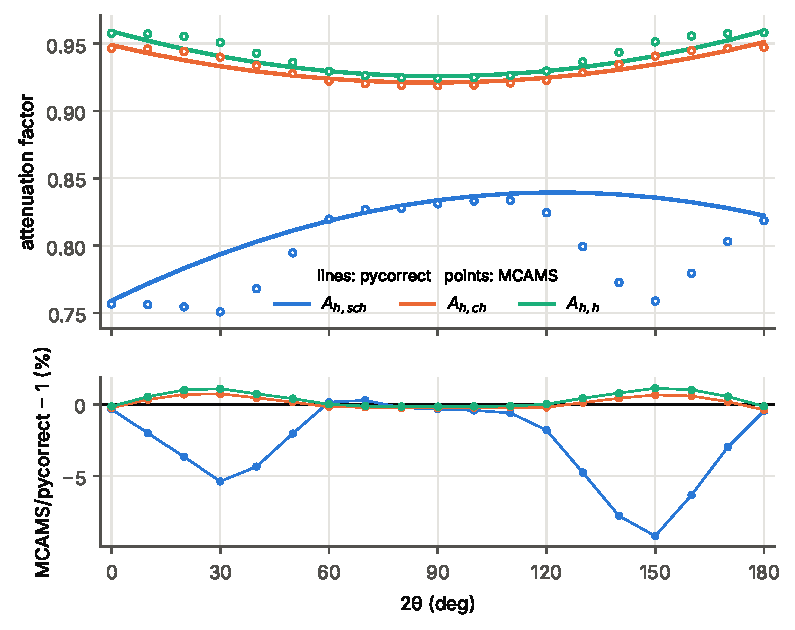
\includegraphics[width=0.82\linewidth]{A4_furnace_factors.pdf}
  \caption{Furnace factors of case A4. The dips of $A_{h,sch}$ near 30$^\circ$ and
  150$^\circ$ are missed by the parabolic interpolation of \cor.}
  \label{fig:A4h}
\end{figure}

\begin{figure}[H]
  \centering
  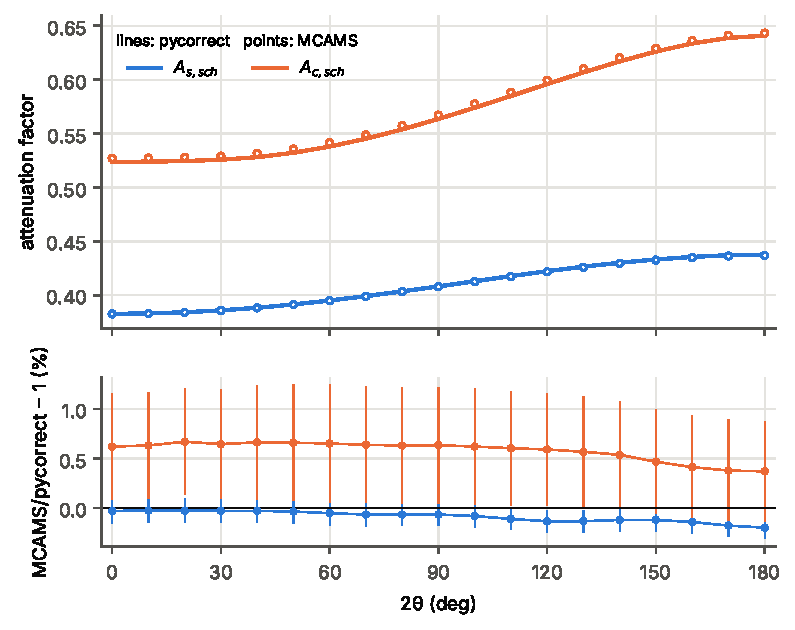
\includegraphics[width=0.82\linewidth]{A4_furnace_sample_can.pdf}
  \caption{Sample and container factors in the presence of the furnace (case A4).}
  \label{fig:A4sc}
\end{figure}

The sample and container factors are unchanged by the furnace and agree
(Figure~\ref{fig:A4sc}). The furnace factors do not (Figure~\ref{fig:A4h}).
Neutrons scattered in the upstream wall of the furnace towards 0--40$^\circ$,
and those scattered in the downstream wall towards 140--180$^\circ$, cross the
sample, which is a strong absorber; the fraction of the wall concerned is
largest near 30$^\circ$ and 150$^\circ$. $A_{h,sch}$ therefore has two deep minima. \cor\ evaluates the
furnace factors only at 0, 90 and 180$^\circ$, where it is exact, and joins them
with a parabola:

\begin{center}\small
\begin{tabular}{@{}llcccc@{}}
\toprule
factor & $2\theta$ & \pyc & \mcams & error & direct sampling \\
\midrule
$A_{h,sch}$ & 0$^\circ$   & 0.75926 & 0.75665 & 0.00175 & 0.75932 \\
            & 30$^\circ$  & 0.79364 & 0.75092 & 0.00195 & 0.75302 \\
            & 90$^\circ$  & 0.83376 & 0.83103 & 0.00195 & 0.83370 \\
            & 150$^\circ$ & 0.83571 & 0.75891 & 0.00176 & 0.76126 \\
            & 180$^\circ$ & 0.82237 & 0.81853 & 0.00202 & 0.82080 \\
\midrule
$A_{h,h}$   & 0$^\circ$   & 0.95907 & 0.95767 & 0.00235 & 0.95907 \\
            & 30$^\circ$  & 0.94053 & 0.95076 & 0.00233 & 0.95216 \\
            & 90$^\circ$  & 0.92576 & 0.92424 & 0.00226 & 0.92578 \\
            & 150$^\circ$ & 0.94072 & 0.95123 & 0.00232 & 0.95259 \\
            & 180$^\circ$ & 0.95935 & 0.95796 & 0.00233 & 0.95936 \\
\bottomrule
\end{tabular}
\end{center}

The \mcams\ values are all about 0.2\% low in this run, which is about one
correlated error bar. A second run with $10^7$ neutrons and other seeds gave
$A_{h,h} = 0.9588, 0.9256, 0.9591$ at 0, 90, 180$^\circ$, within 0.03\% of the
direct sampling.

\begin{warn}[Consequence]
The furnace contribution subtracted from the sample is $A_{h,sch}I_h/A_{s,sch}$.
An error of up to 9\% in $A_{h,sch}$ over the angular ranges 10--50$^\circ$ and
120--170$^\circ$ leaves a structured residue of furnace scattering in the result.
\end{warn}

% =========================================================================
\chapter{Multiple scattering: results}
\label{chap:ms}
% =========================================================================

\section{The double-scattering table (B1)}

\begin{figure}[H]
  \centering
  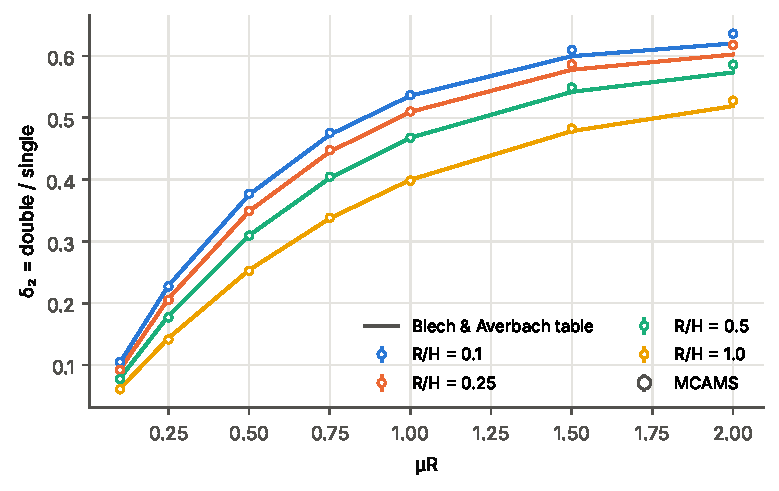
\includegraphics[width=0.82\linewidth]{B1_delta2.pdf}
  \caption{Double-to-single ratio $\delta_2$ for a pure scatterer: Blech \&
  Averbach table, interpolated as in \pyc\ (lines), and \mcams\ (points).}
  \label{fig:B1}
\end{figure}

\begin{center}\small
\begin{tabular}{@{}c cc cc cc cc@{}}
\toprule
 & \multicolumn{2}{c}{$R/H=0.1$} & \multicolumn{2}{c}{$R/H=0.25$} & \multicolumn{2}{c}{$R/H=0.5$} & \multicolumn{2}{c}{$R/H=1$} \\
$\mu R$ & table & MC & table & MC & table & MC & table & MC \\
\midrule
0.10 & 0.1042 & 0.1042 & 0.0927 & 0.0918 & 0.0788 & 0.0771 & 0.0619 & 0.0607 \\
0.25 & 0.2285 & 0.2318 & 0.2075 & 0.2052 & 0.1796 & 0.1771 & 0.1435 & 0.1412 \\
0.50 & 0.3757 & 0.3770 & 0.3489 & 0.3493 & 0.3096 & 0.3095 & 0.2538 & 0.2526 \\
0.75 & 0.4726 & 0.4727 & 0.4451 & 0.4476 & 0.4026 & 0.4047 & 0.3373 & 0.3384 \\
1.00 & 0.5358 & 0.5370 & 0.5095 & 0.5102 & 0.4678 & 0.4676 & 0.3997 & 0.3984 \\
1.50 & 0.5997 & 0.6067 & 0.5777 & 0.5863 & 0.5420 & 0.5490 & 0.4785 & 0.4827 \\
2.00 & 0.6204 & 0.6330 & 0.6025 & 0.6176 & 0.5734 & 0.5861 & 0.5190 & 0.5278 \\
\bottomrule
\end{tabular}
\end{center}

The table is confirmed: the differences are below 1\% up to $\mu R = 1$, apart
from the smallest values ($\mu R \leq 0.25$, $R/H \geq 0.5$), where they reach
2.2\% (absolute differences below 0.003). They grow to 1.5--2.5\% at $\mu R = 1.5$--2, with
\mcams\ always higher. The typical statistical error is 0.1--0.4\% of the value.

\section{Higher orders (B1, B2)}

\begin{figure}[H]
  \centering
  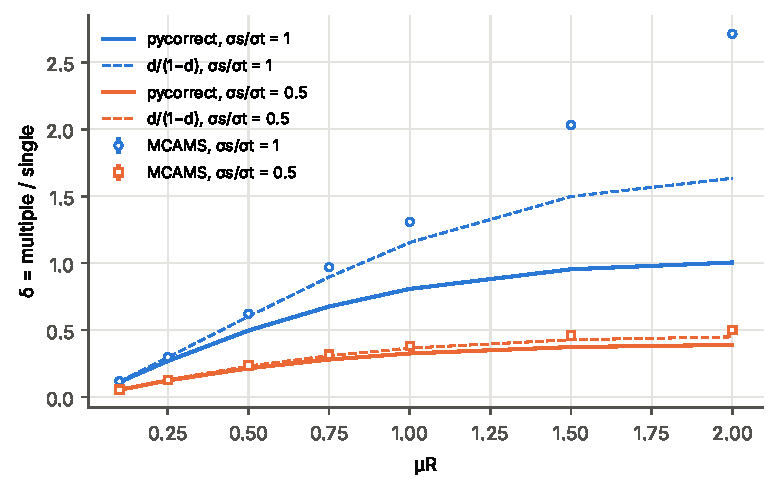
\includegraphics[width=0.82\linewidth]{B2_delta_total.pdf}
  \caption{Total multiple-scattering ratio $\delta$ (all orders) for $R/H=0.1$:
  \pyc\ (solid), \mcams\ (points) and the geometric series $d/(1-d)$ (dashed),
  for a pure scatterer and for $\sigma_s/\sigma_t=0.5$.}
  \label{fig:B2}
\end{figure}

Although $d$ is correct, the total $\delta$ of \pyc\ is too small, and the
difference grows quickly with $\mu R$ (Figure~\ref{fig:B2}):

\begin{center}\small
\begin{tabular}{@{}c ccc ccc@{}}
\toprule
 & \multicolumn{3}{c}{$\sigma_s/\sigma_t = 1$} & \multicolumn{3}{c}{$\sigma_s/\sigma_t = 0.5$} \\
$\mu R$ & \pyc & \mcams & $d/(1-d)$ & \pyc & \mcams & $d/(1-d)$ \\
\midrule
0.10 & 0.112 & 0.116 & 0.116 & 0.054 & 0.056 & 0.055 \\
0.25 & 0.270 & 0.303 & 0.296 & 0.124 & 0.129 & 0.129 \\
0.50 & 0.497 & 0.624 & 0.602 & 0.215 & 0.236 & 0.231 \\
0.75 & 0.676 & 0.958 & 0.896 & 0.281 & 0.317 & 0.309 \\
1.00 & 0.808 & 1.314 & 1.154 & 0.326 & 0.380 & 0.366 \\
1.50 & 0.954 & 2.010 & 1.498 & 0.374 & 0.459 & 0.428 \\
2.00 & 1.005 & 2.706 & 1.635 & 0.390 & 0.502 & 0.450 \\
\bottomrule
\end{tabular}
\end{center}

The reason is visible order by order. The series~(\ref{eq:series}) assumes that
the third order is $0.694\,d$ times the second. In the simulation the ratio of
successive orders is $(1.03$--$1.2)\,\delta_2$ (Figure~\ref{fig:ratio}),
slowly increasing with $\mu R$ above $\mu R = 0.5$. Each further scattering is about as likely as
the previous one: the neutrons that have scattered twice are, on average, deeper
in the sample. A geometric series, $\delta \approx d/(1-d)$, is a much better
approximation for $\mu R \lesssim 0.75$ and for absorbing samples. For strongly
scattering, thick samples only a full calculation is reliable.

\begin{figure}[H]
  \centering
  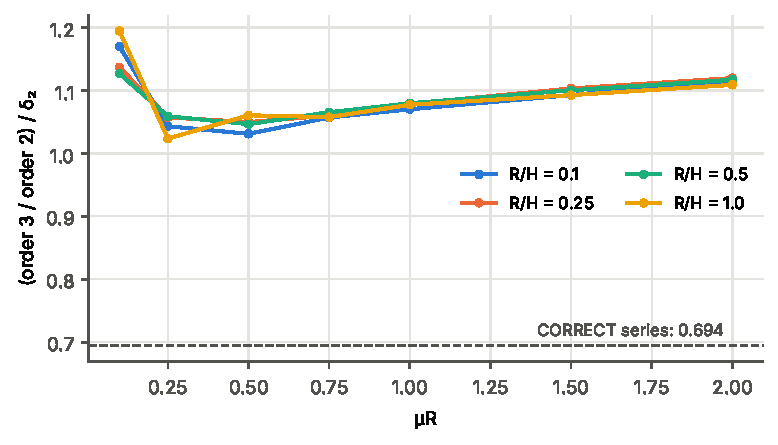
\includegraphics[width=0.82\linewidth]{B2_order_ratio.pdf}
  \caption{Ratio of third to second order divided by $\delta_2$, from \mcams.
  The series of \cor\ assumes 0.694.}
  \label{fig:ratio}
\end{figure}

\section{Angle dependence and the container (B3)}

\begin{figure}[H]
  \centering
  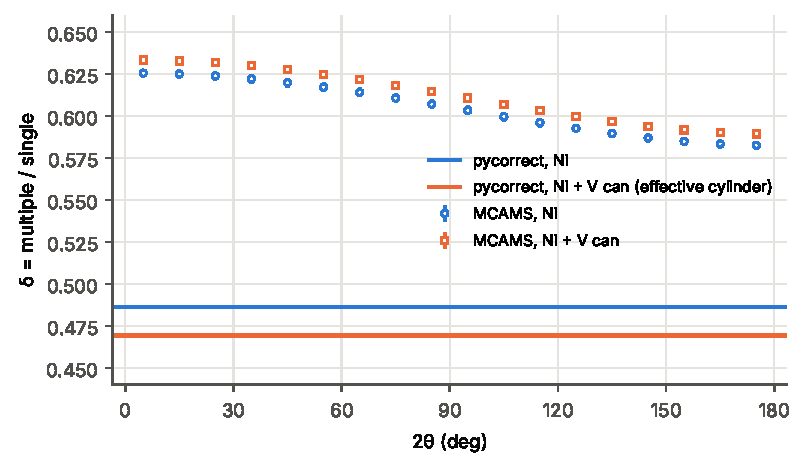
\includegraphics[width=0.82\linewidth]{B3_angle.pdf}
  \caption{$\delta(2\theta)$ for the Ni sample alone and in its V can, $H = 3$~cm.
  Horizontal lines: the constant values of \pyc.}
  \label{fig:B3}
\end{figure}

For the Ni sample ($\mu R = 0.54$, $\sigma_s/\sigma_t = 0.937$, $R/H = 0.1$)
\mcams\ gives $\delta$ from 0.625 at low angles to 0.583 at 175$^\circ$ (mean
0.605). \pyc\ gives a constant 0.486, or 0.501 with \code{faithful on}. With
the can, \mcams\ gives a slightly \emph{larger} $\delta$ (0.589--0.633), while
the effective cylinder of \cor\ gives a smaller one (0.469). The dominant error
is that of the series. On the cross-section it amounts to
$\Delta\delta\,\sigma_s/4\pi \approx 0.12 \times 1.47 = 0.17$~b\,sr$^{-1}$,
about 12\% of the self-scattering level of Ni. The vanadium normalisation,
outside the scope of this report, may partly compensate it through $\delta_v$, which is also underestimated.

\section{Sample taller than the beam (B4)}

\begin{figure}[H]
  \centering
  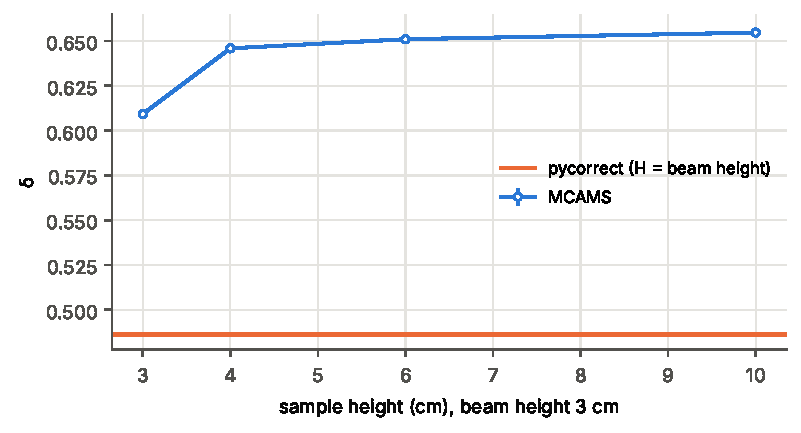
\includegraphics[width=0.75\linewidth]{B4_tall_sample.pdf}
  \caption{$\delta$ (angle average) for the Ni rod as a function of the sample
  height, for a 3~cm high beam.}
  \label{fig:B4}
\end{figure}

\cor\ uses the beam height for $H$. A real sample is usually taller than the
beam, and neutrons scattered out of the beam can be scattered back. $\delta$
increases from 0.609 (sample height = beam height) to 0.646 for a 4~cm sample
and 0.655 for a 10~cm sample: most of the effect comes from the first
centimetre above and below the beam.

\section{The complete D4 example}

The function \code{mcams_factors_like_pycorrect} takes the state of a \pyc\ run
and computes all its factors with \mcams\ on the same $2\theta$ grid
(Chapter~\ref{chap:howto}). For the D4 example of the \pyc\ manual (Ni in a V
can, V rod, beam $5\times1.5$~cm):

\begin{figure}[H]
  \centering
  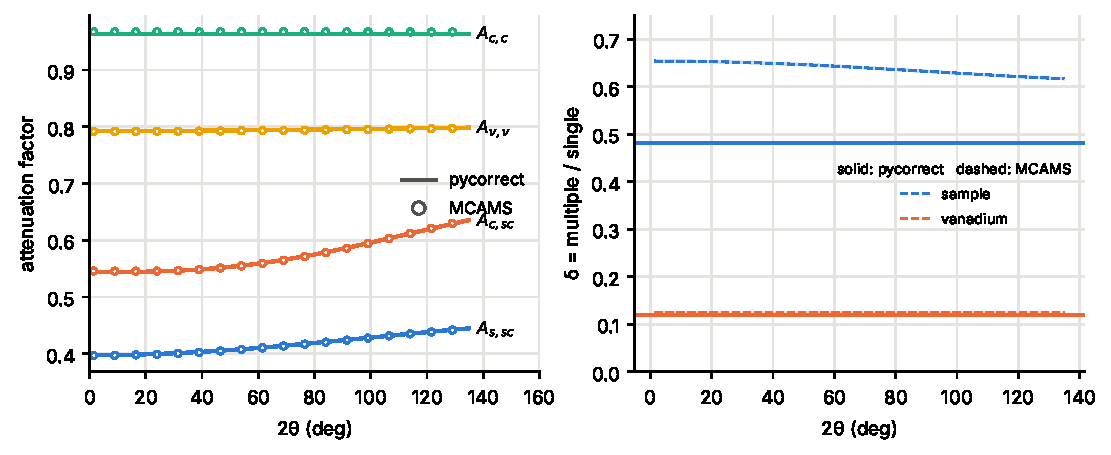
\includegraphics[width=\linewidth]{D4_example.pdf}
  \caption{D4 example. Left: attenuation factors of sample, can and vanadium
  (lines \pyc, points \mcams). Right: $\delta$ of sample and vanadium.}
\end{figure}

The attenuation factors agree within 0.4\%, and $\delta_v$ of the vanadium rod
($\mu R = 0.14$) within 4\% (0.120 against 0.125). For the sample, $\delta_s =
0.482$ in \pyc\ against 0.62--0.65 in \mcams.

% =========================================================================
\chapter{Partially filled samples and offset layers}
\label{chap:vertical}
% =========================================================================

Up to version 2.1 every layer of \mcams\ started at the bottom of the sample,
and a partial fill was described by the level of the material only. Version~2.2
gives each layer its own vertical band, $b_i \le y \le b_i + h_i$, measured from
the centre of the beam ($y = 0$). The powder can now rest on a support above the
bottom of the beam, and the container can start inside the beam. This chapter
uses that feature to test the \emph{fullness} correction of \cor.

\section{What CORRECT does}

With \code{sample ... /fullness=f}, \cor\ assumes that the fraction $f$ of the
beam height sees the full container and the fraction $1-f$ sees the empty one.
Before the Paalman \& Pings step it replaces the measured sample intensity by the
intensity of a full container:
\begin{equation}
  I_{sc,\mathrm{full}} = \frac{I_{sc} - (1-f)\,I_c}{f},
  \label{eq:fullness}
\end{equation}
and then continues as for a full container: $I_s = (I_{sc,\mathrm{full}} -
A_{c,sc} I_c/A_{c,c})/A_{s,sc}$, with the factors of the full can, and the
multiple-scattering correction $\delta_C$ from \code{mscat} with the full beam
height. (The fullness step is applied before the background subtraction;
the result is the same because the background enters
equation~(\ref{eq:fullness}) with total weight 1.)

Equation~(\ref{eq:fullness}) is exact for single scattering if
\begin{itemize}
  \item the scattering detected in the horizontal plane comes from the same
        height at which the neutron entered (true for single scattering:
        incoming and outgoing paths are horizontal);
  \item the beam intensity does not depend on $y$, so that $f$, a fraction of
        height, is also a fraction of the flux;
  \item the container covers the whole beam height.
\end{itemize}
It does not matter \emph{where} the powder is inside the beam: only the fraction
of the beam height that it covers enters. The tests below check each condition.

\section{How the comparison is done}

The script \file{compare\_vertical\_extent.py} builds the geometries with
\mcams~2.2 and simulates, at exact detector angles, the intensity per incident
neutron and per steradian of the sample in its can ($I_{sc}$) and of the empty
can ($I_c$), split into single and multiple scattering. These ``measurements''
are processed with exactly the steps above, using the \pyc\ functions
\code{atcors}, \code{plate} and \code{mscat}. The result is compared with the true
single scattering $I_\mathrm{true}$ of a sample that fills the whole beam height,
without attenuation:
\begin{equation}
  e(2\theta) = \frac{I_s}{I_\mathrm{true}} - 1 - \delta_C .
\end{equation}
$e$ is the error left in the corrected cross section, in units of the single
scattering. It is split into
\begin{itemize}
  \item $e_\mathrm{single}$: the same steps applied to the single-scattering
        part only. It tests the fullness step and the attenuation factors.
  \item $\delta_\mathrm{eff}$: the multiple scattering left after the steps.
        This is what \cor\ should subtract; compare it with $\delta_C$.
\end{itemize}

\paragraph{Geometry.} Ni powder (radius 3~mm, $\mu = 0.180$~mm$^{-1}$,
$\sigma_s/\sigma_t = 0.937$) in a V can (wall 0.2~mm, $\mu =
0.0459$~mm$^{-1}$), beam $15 \times 20$~mm ($-10 \le y \le 10$), can from
$y=-30$ to $+30$~mm unless stated. Flat cell: V windows of 0.2~mm, 2~mm of Ni,
40~mm wide, normal incidence. Each case uses 8 independent runs of $10^5$
neutrons; the errors are the standard errors of the mean. They are strongly
correlated from angle to angle, because every angle uses the same trajectories.

\begin{center}\small
\begin{tabularx}{\linewidth}{@{}l>{\raggedright\arraybackslash}Xc@{}}
\toprule
Case & Powder (and can) & $f$ \\
\midrule
V1 & powder from the can bottom ($-30$) up to $+10$, $+5$, $0$, $-5$~mm & 1, 0.75, 0.5, 0.25 \\
V2 & powder band from $+2$ to $+30$~mm, resting on a support (empty can below it) & 0.40 \\
V3 & can from $-5$ to $+55$~mm (bottom inside the beam), powder from $-5$ to $+3$ & 0.40 \\
V4 & as V1 with level $-4$~mm, Gaussian vertical beam profile ($\sigma = 5$~mm) & 0.30 \\
Slab & flat cell, Ni from $-30$ up to $+10$ and $0$~mm & 1, 0.5 \\
\bottomrule
\end{tabularx}
\end{center}

In \mcams~2.2 the sample of case V2, for example, is
\begin{lstlisting}
from cylinder import create_cylindrical_sample
from sample_base import Layer
sample = create_cylindrical_sample(None, [               # height: envelope of the layers
    Layer("Ni", 6.0, 0.18027, 0.937, bottom=2.0,   height=28.0),
    Layer("V",  0.2, 0.04591, 0.7785, bottom=-30.0, height=60.0)],
    beam_height=20.0)
print(sample.beam_fullness())     # [0.4, 1.0]: the f to give to CORRECT
\end{lstlisting}

\section{Single scattering}

\begin{figure}[H]
  \centering
  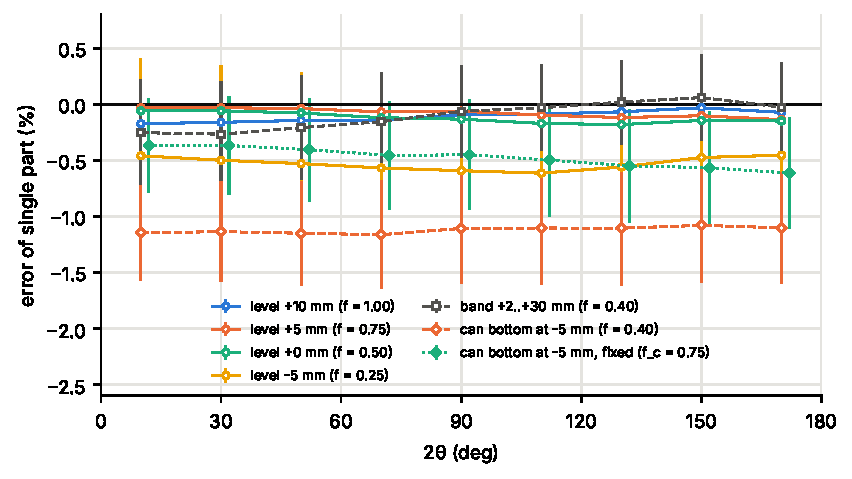
\includegraphics[width=0.92\linewidth]{V_single_residual.pdf}
  \caption{Error of the single-scattering part after the fullness step and the
  Paalman \& Pings correction of \cor, cylinder cases V1--V3. The green
  diamonds use the fixed recipe of equation~(\ref{eq:fixed}) for case V3.}
  \label{fig:Vsingle}
\end{figure}

\begin{itemize}
  \item \textbf{Powder level inside the beam (V1).} $e_\mathrm{single}$ is
        within $\pm0.2\%$ for $f = 1$, 0.75 and 0.5, and $-0.5 \pm 0.8\%$ for
        $f = 0.25$. The fullness step is exact, as expected.
  \item \textbf{Powder resting on a support (V2).} The empty part is now
        \emph{below} the powder; $e_\mathrm{single}$ is within $\pm0.3\%$. The
        step depends only on $f$, not on where the powder is.
  \item \textbf{Can bottom inside the beam (V3).} The lowest quarter of the beam
        misses the can, and \cor\ is wrong by $-1.1\%$. The measured empty can
        has only $f_c = 0.75$ of the full-height can, so the step subtracts too
        much. The correct recipe is
        \begin{equation}
          I_{sc,\mathrm{full}} = \frac{I_{sc} - \frac{f_c - f}{f_c}\,I_c}{f},
          \qquad I_{c,\mathrm{full}} = \frac{I_c}{f_c},
          \label{eq:fixed}
        \end{equation}
        with $I_{c,\mathrm{full}}$ used in the Paalman \& Pings step. It brings
        the error to $-0.5 \pm 0.5\%$. The size of the error depends on how
        much the can scatters: here the V wall is thin, and the error is small.
\end{itemize}

\paragraph{Non-uniform beam (V4).} \cor's $f$ is a fraction of the beam
\emph{height}. If the beam is not uniform, the right fraction is the fraction of
the \emph{flux}:
\begin{equation}
  f_\mathrm{eff} = \frac{\int_{\text{material}} V(y)\,\deriv{y}}
                        {\int_{\text{beam}} V(y)\,\deriv{y}} .
\end{equation}
For a Gaussian profile with $\sigma = 5$~mm and the powder level at $-4$~mm the
geometric fraction is 0.30 and $f_\mathrm{eff} = 0.198$. With the geometric $f$
the cross section is 33\% too low; with $f_\mathrm{eff}$ the error is $-0.3 \pm
0.8\%$ (Figure~\ref{fig:Vprofile}). The error is $f_\mathrm{eff}/f - 1$, the
same at all angles, so it looks like a normalisation error.

\begin{figure}[H]
  \centering
  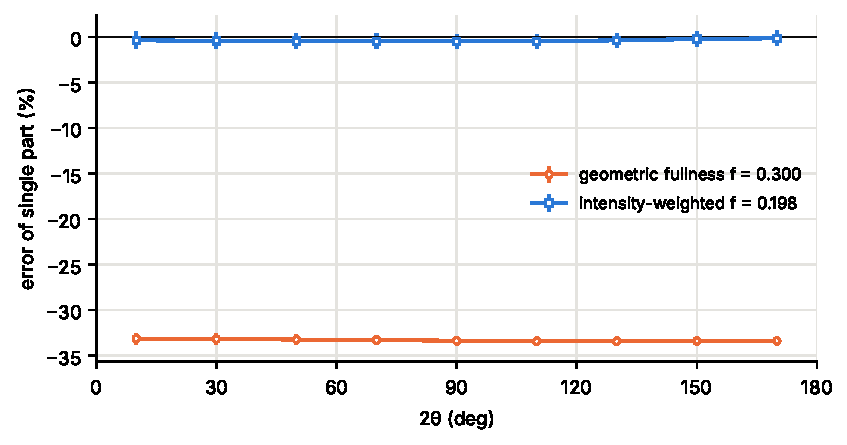
\includegraphics[width=0.85\linewidth]{V_profile.pdf}
  \caption{Gaussian beam profile (case V4): fullness as a fraction of height
  and as a fraction of flux.}
  \label{fig:Vprofile}
\end{figure}

\section{Multiple scattering}

\begin{figure}[H]
  \centering
  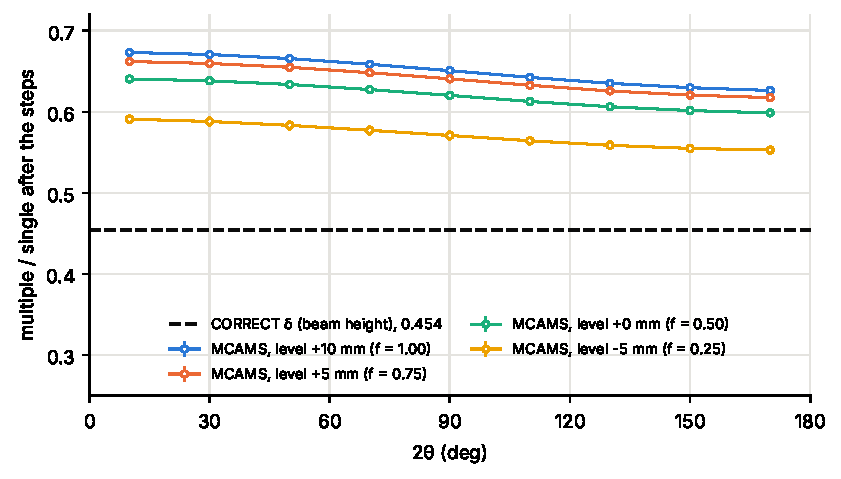
\includegraphics[width=0.92\linewidth]{V_multiple.pdf}
  \caption{Multiple scattering left after the fullness step and the Paalman \&
  Pings correction, in units of the single scattering ($\delta_\mathrm{eff}$),
  and the $\delta_C$ that \cor\ subtracts (case V1).}
  \label{fig:Vmult}
\end{figure}

\cor\ subtracts the same $\delta_C = 0.454$ for every fullness: \code{mscat} is
called with the full beam height and the volume-averaged $\mu$ of sample and can.
\mcams\ gives $\delta_\mathrm{eff}$ from 0.67--0.63 for a full can to
0.59--0.55 for $f = 0.25$ (Figure~\ref{fig:Vmult}). Two effects combine:
\begin{itemize}
  \item the higher orders of the series are too low (Chapter~\ref{chap:ms}), which makes
        $\delta_C$ too small for any fullness;
  \item a partial fill reduces the multiple scattering, because there is less
        powder near the beam. The powder below the beam still contributes,
        so the reduction is much smaller than $f$ itself.
\end{itemize}
After the full \cor\ chain the remaining error $e$ is +17 to +22\% for $f=1$,
+9 to +13\% for $f = 0.25$, +14 to +17\% for the powder band (V2), and +4 to
+7\% for the can that starts inside the beam (V3). The complete tables are in
\file{results/V\_cylinder.txt}.

\section{Flat cell and the PLATE bug}

For the flat cell \cor\ uses \code{plate} for the attenuation factors and
makes no multiple-scattering correction. The comparison showed an error of
$-1.8\%$ in $e_\mathrm{single}$ at $2\theta = 110^\circ$, decreasing to
$-0.6\%$ at $170^\circ$, in reflection geometry only. A check of \code{plate}
against the direct method of \mcams~2.1 found two errors in the Fortran
subroutine \code{PLATE}:
\begin{enumerate}
  \item \textbf{Reflection geometry, $A_{c,sc}$.} For neutrons scattered in the
        back window, \cor\ includes the attenuation of the sample on the way in
        only. On the way out the scattered neutron crosses the sample again.
        The correct factor is
        \begin{equation}
          A_{c,sc}^{(2)} = e^{(\mu_c d + \mu_s t)(b-a)}\,A_{c,sc}^{(1)},
        \end{equation}
        with $a = 1/\cos\phi$, $b = 1/\cos(2\theta-\phi)$ ($b<0$ in reflection),
        instead of $e^{\mu_c d (b-a)} e^{-\mu_s t a} A_{c,sc}^{(1)}$. For this
        cell \cor\ gives $A_{c,sc} = 0.821$ at $110^\circ$; the correct value is
        0.606.
  \item \textbf{Transmission with $a = b$} ($2\theta = 0$ at normal incidence),
        $A_{c,c}$: the two windows are added but not averaged, and the factor
        is 2 times too large (1.964 instead of 0.982).
\end{enumerate}
Both are now corrected in \pyc\ (\code{faithful=False}, the default);
\code{faithful=True} keeps the original formulas.

\begin{center}\small
\begin{tabular}{@{}lcccc@{}}
\toprule
& \multicolumn{2}{c}{level $+10$~mm ($f=1$)} & \multicolumn{2}{c}{level $0$~mm ($f=0.5$)} \\
$2\theta$ & corrected \code{plate} & \cor\ 2.24 & corrected \code{plate} & \cor\ 2.24 \\
\midrule
$30^\circ$  & $+0.01 \pm 0.14\%$ & $+0.01\%$ & $-0.36 \pm 0.16\%$ & $-0.36\%$ \\
$110^\circ$ & $-0.02 \pm 0.10\%$ & $-1.80\%$ & $-0.23 \pm 0.31\%$ & $-2.00\%$ \\
$150^\circ$ & $-0.01 \pm 0.11\%$ & $-0.73\%$ & $-0.27 \pm 0.23\%$ & $-0.99\%$ \\
\bottomrule
\end{tabular}

\smallskip
$e_\mathrm{single}$ for the flat cell (\file{results/V\_slab.txt}).
\end{center}

With the corrected \code{plate} the fullness step is exact for the flat cell
too (within 2 standard errors). The multiple scattering of the cell, which
\cor\ does not correct, is $\delta_\mathrm{eff} = 0.51$--$0.56$: a flat
sample much wider and taller than its thickness has a lot of multiple
scattering in its plane.

\begin{note}[Summary for partially filled samples]
\begin{itemize}
  \item The fullness step of \cor\ is exact for single scattering, for
        cylinders and plates, wherever the powder is inside the beam, if the
        can covers the whole beam and the beam is uniform. Give \cor\ the
        value of \code{sample.beam_fullness()} from \mcams.
  \item If the can bottom is inside the beam, use equation~(\ref{eq:fixed}).
  \item If the beam is not uniform, use the flux fraction $f_\mathrm{eff}$.
        The geometric fraction can be wrong by tens of per cent.
  \item The multiple-scattering correction does not depend on the fullness in
        \cor; it does in reality. Take $\delta(2\theta)$ from \mcams\ for the
        real geometry.
\end{itemize}
\end{note}

% =========================================================================
\chapter{Conclusions}
% =========================================================================

\begin{enumerate}
  \item \textbf{The two codes agree} where the physics is the same: attenuation
        factors for a beam wider than the sample, and the Blech \& Averbach
        double-scattering ratio. This validates both the translation of \cor\ and
        the Monte Carlo transport of \mcams.
  \item \textbf{Narrow beams}: \cor's quadrature is about 1\% wrong for a beam
        narrower than the sample. Use \mcams, or improve \code{atcors} (more Gauss
        panels), when the beam is narrower than the sample.
  \item \textbf{Furnaces and cryostats}: the parabolic interpolation of the
        furnace factors is a serious approximation; errors reach 9\% in
        $A_{h,sch}$ where the scattered beam crosses the sample. Compute the
        furnace factors at all angles (\mcams, or \code{atcors} at more angles).
  \item \textbf{Multiple scattering}: the table is good but the series for the
        higher orders is not. \cor\ underestimates $\delta$ by 20--40\% for
        typical samples ($\mu R \approx 0.5$--1, weak absorption). It also
        ignores the angle dependence and the sample height above and below the
        beam. Replacing the series by $d/(1-d)$ is a cheap improvement; the
        \mcams\ value of $\delta(2\theta)$ is the accurate one.
  \item \textbf{Partial fill}: the fullness step is exact for single
        scattering when the can covers the whole beam and the beam is uniform,
        for cylinders and plates. Otherwise use the fixed recipe
        (equation~\ref{eq:fixed}) and the flux fraction $f_\mathrm{eff}$.
        \mcams~2.2 gives $f$ directly (\code{sample.beam_fullness()}) and the
        true $\delta(2\theta)$ of the partially filled sample.
  \item \textbf{Flat plates}: use \pyc\ with \code{faithful=False} (the
        default); the original \code{PLATE} is wrong in reflection geometry by
        up to 2\% in the corrected cross section of the test cell.
  \item \textbf{Recommended use}: keep \pyc\ for the data reduction chain. For
        thick or strongly scattering samples, narrow beams and furnaces, take the
        attenuation factors and $\delta(2\theta)$ from \mcams\ for the same
        geometry (Chapter~\ref{chap:howto}).
\end{enumerate}

\begin{warn}[Limits of this comparison]
Both programs assume isotropic scattering for multiple scattering, ignore
inelasticity in the multiple-scattering terms, and treat the sample as
homogeneous. The comparison tests the implementations and the approximations of
\cor, not these common assumptions. No measured data were used.
\end{warn}

% =========================================================================
\chapter{How to use MCAMS to do what pycorrect does}
\label{chap:howto}
% =========================================================================

\section{Where things are}

\begin{lstlisting}[style=shell]
parent/
  MCAMS/        beam.py, cylinder.py, transmission_by_layer.py, ...
  pycorrect/    pycorrect package (pip install -e .)
  comparison/   pyc_mcams_bridge.py, compare_pycorrect_mcams.py,
                example_d4_with_mcams.py, report/
\end{lstlisting}
If the folders are elsewhere, set \code{MCAMS_DIR} and \code{PYCORRECT_DIR}.

\section{Step 1 -- the sample in MCAMS}

Convert the \pyc\ geometry to \mcams\ layers: diameter for the inner layer, radial
thicknesses for the others, mm and mm$^{-1}$.

\begin{lstlisting}
import pyc_mcams_bridge as br          # puts MCAMS and pycorrect on sys.path
from cylinder import create_cylindrical_sample      # MCAMS

lam = 0.4985
mu_ni = br.mu_total(0.0913, 18.5, 4.49, lam)       # 1/cm, as pycorrect
mu_v  = br.mu_total(0.0722, 4.95, 5.08, lam)
layers, names = br.cylinder_layers_from_pycorrect(
    r1=0.30, r2=0.32,                 # cm: sample radius, can outer radius
    smu=mu_ni, cmu=mu_v,              # 1/cm
    s_frac=0.937, c_frac=0.779)       # mu_s/mu_t (for multiple scattering)
sample = create_cylindrical_sample(50.0, layers)    # height in mm
print(sample.summary())
\end{lstlisting}
or directly in \mcams\ units:
\begin{lstlisting}
sample = create_cylindrical_sample(50.0, [("Ni", 6.0, 0.18027, 0.937),
                                          ("V",  0.2, 0.04591, 0.779)])
\end{lstlisting}
The layer builder of \mcams\ (\code{layer_builder.py}) can also compute $\mu$
from a chemical formula and a density. To compare with \pyc, use the same cross
sections in both.

\section{Step 2 -- Paalman \& Pings factors}

\begin{lstlisting}
import math, numpy as np
from transmission_by_layer import transmission_by_last_layer   # MCAMS
from pycorrect.ndplib import area

W, Hb = 15.0, 20.0                       # beam width and height (mm)
angles = np.arange(0, 181, 5.0)
pure = create_cylindrical_sample(50.0, [("Ni", 6.0, 0.18027, 1.0),
                                        ("V",  0.2, 0.04591, 1.0)])
res = transmission_by_last_layer(pure, W, Hb, n_particles=400_000,
                                 angles_deg=angles, max_orders=1, rng=1)
S_single = res.sum_attenuation[0] / res.n_incident   # (layers, angles)
# unattenuated rate mu_k S_k / W  (S_k: part of layer k inside the beam)
S_ni = area(3.0, W / 2)
S_v  = area(3.2, W / 2) - area(3.0, W / 2)
A_ssc = S_single[0] / (0.18027 * S_ni / W)          # = pycorrect assch
A_csc = S_single[1] / (0.04591 * S_v / W)           # = pycorrect acsch
\end{lstlisting}

\begin{itemize}
  \item Use scatter fraction 1 for this step: it does not change $A$ but gives
        more events. Use \code{max_orders=1}: only first scatterings enter $A$.
  \item The beam must be lower than the sample, so that neutrons scattered
        horizontally leave through the side.
  \item For $A_{c,ch}$ run again with $\mu=0$ in the sample layer; for $A_{h,h}$
        with $\mu=0$ in sample and can.
  \item \code{br.mc_attenuation_factors(layers, beam_width_cm, angles)} does all
        this and also returns error bars from independent runs.
\end{itemize}

\section{Step 3 -- multiple scattering}

\begin{lstlisting}
H = 30.0                                  # mm; sample height = beam height (CORRECT)
s = create_cylindrical_sample(H, [("Ni", 6.0, 0.18027, 0.937)])
res = transmission_by_last_layer(s, 8.0, H, n_particles=100_000,
                                 angles_deg=angles, rng=2)
single   = res.sum_attenuation[0].sum(axis=0)     # all layers
multiple = res.sum_attenuation[1].sum(axis=0)
delta = multiple / single                         # delta(2theta), replaces mscat()
\end{lstlisting}
Give the real sample height instead of $H$ to include the sample above and below
the beam. \code{br.mc_delta(...)} returns $\delta$, $\delta_2$ and the ratio of
orders, with errors.

\section{Step 4 -- all the factors of a pycorrect run at once}

\begin{lstlisting}
from pycorrect import Correct
import pyc_mcams_bridge as br

c = Correct(verbose=False, ask=False)
c.run_file("d4_example.com")              # pycorrect, as usual
r = c.results[0]
mc = br.mcams_factors_like_pycorrect(c.st, r["theta"])
# same names as pycorrect: mc["assch"], mc["acsch"], mc["acch"], mc["ahsch"],
# mc["ahch"], mc["ahh"], mc["avvch"], mc["delta_sa"], mc["delta_va"]
# (+ "<name>_err"); delta_* are arrays versus 2theta
\end{lstlisting}

\section{Step 5 -- correcting data with the MCAMS factors}

The subtraction scheme of \cor\ is unchanged; only the factors are replaced.
For data $I_{sch}, I_{ch}, I_h$ (background already subtracted) on the grid
\code{theta}:

\begin{lstlisting}
I_h = I_h_raw / mc["ahh"]
I_c = (I_ch - mc["ahch"] * I_h) / mc["acch"]
I_s = (I_sch - mc["acsch"] * I_c - mc["ahsch"] * I_h) / mc["assch"]
# ... normalisation with the vanadium (pycorrect), then
# dcs = normalised - mc["delta_sa"] * sigma_s / (4 * np.pi) + P_s
\end{lstlisting}

\section{Step 6 -- partially filled samples (MCAMS 2.2)}

Describe each layer with its own band, measured from the beam centre, and let
\mcams\ give the fullness for \pyc:
\begin{lstlisting}
from sample_base import Layer
sample = create_cylindrical_sample(None, [
    Layer("Ni", 6.0, 0.18027, 0.937,  bottom=-30.0, height=30.0),   # powder up to y = 0
    Layer("V",  0.2, 0.04591, 0.7785, bottom=-30.0, height=60.0)],  # the can
    beam_height=20.0)
f = sample.beam_fullness()[0]          # 0.5 -> sample ... /fullness=0.5 in pycorrect
res = transmission_by_last_layer(sample, 15.0, 20.0, n_particles=100_000,
                                 angles_deg=angles, rng=3)
\end{lstlisting}
\code{beam_fullness} is a fraction of the beam height; for a non-uniform beam
use the flux fraction (Chapter~\ref{chap:vertical}). The point estimator then
gives the true $\delta(2\theta)$ of the partially filled sample. From the
command line, the main script of \mcams\ does the same for the layers named in
\code{CONTENT_LAYERS}: \code{python run_simulation.py --geometry cylinder --bottom -30 --height 30}.

\section{Practical advice}

\begin{itemize}
  \item \textbf{Statistics.} $4\times10^5$ neutrons give $A_s$ to 0.1\% and thin
        containers to 0.5\%. Thin walls receive few interactions: increase the
        number of neutrons for container and furnace factors.
  \item \textbf{Angles.} Compute every 5--10$^\circ$ and interpolate. The furnace
        factors need at least 5$^\circ$ steps to resolve their dips.
  \item \textbf{Run time.} Attenuation (first order only) takes seconds.
        Multiple scattering takes longer for weakly absorbing, thick samples
        (many orders).
  \item \textbf{Consistency.} Use the same $\mu$ in both programs
        (\code{br.mu_total} reproduces the formula of \pyc), the same beam
        width, and, for multiple scattering, the same height.
\end{itemize}

% =========================================================================
\chapter{Running the comparison}
% =========================================================================

\begin{lstlisting}[style=shell]
cd comparison
python compare_pycorrect_mcams.py           # parts A, B, C   (about 4 minutes)
python compare_pycorrect_mcams.py --quick   # fewer neutrons  (about 20 s)
python compare_pycorrect_mcams.py --part b  # only multiple scattering
python compare_pycorrect_mcams.py --replot  # redraw the attenuation figures
python example_d4_with_mcams.py             # the D4 example (about 15 s)
python compare_vertical_extent.py           # partial fill, chapter 6 (about 30 s)
cd report && latexmk -pdf main.tex          # this report
\end{lstlisting}

\begin{center}\small
\begin{tabularx}{\linewidth}{@{}l>{\raggedright\arraybackslash}X@{}}
\toprule
File & Content \\
\midrule
\file{results/A*\_*.txt}, \file{.npz} & attenuation factors: $2\theta$, \pyc, \mcams, error for each factor \\
\file{results/B1\_delta2\_RH*.txt} & $\mu R$, table, MC $\delta_2$, error, \pyc\ $\delta$, MC $\delta$, error, order ratio \\
\file{results/B2\_absorbing.txt} & the same for $\sigma_s/\sigma_t = 0.5$ \\
\file{results/B3\_angle\_dependence.txt} & $\delta(2\theta)$ of Ni and Ni in V can \\
\file{results/B4\_tall\_sample.txt} & $\delta$ against sample height \\
\file{results/C\_independent\_check.txt} & direct-sampling check of the disputed values \\
\file{results/D4\_example.txt} & all factors of the D4 example \\
\file{results/V\_cylinder.txt}, \file{V\_slab.txt} & partial fill: $e_\mathrm{single}$, $\delta_\mathrm{eff}$, $e$ with errors, for every case \\
\file{figures/*.pdf} & the figures of this report \\
\bottomrule
\end{tabularx}
\end{center}

% =========================================================================
\appendix
\chapter{Functions of \texttt{pyc\_mcams\_bridge.py}}
% =========================================================================

\begin{fnbox}{cm\_to\_mm(x), per\_cm\_to\_per\_mm(mu), mu\_total(rho, sigma\_s, sigma\_a, wavelength)}
Unit conversion, and $\mu = n(\sigma_s + \sigma_a\lambda/1.798)$ in cm$^{-1}$ as in \pyc.
\end{fnbox}

\begin{fnbox}{cylinder\_layers\_from\_pycorrect(r1, r2, r3, r4, smu, cmu, hmu, s\_frac, c\_frac, h\_frac)}
\mcams\ layers equivalent to the arguments of \code{atcors}: sample (diameter),
can, gap ($\mu=0$), furnace. Returns \code{(layers, names)}.
\end{fnbox}

\begin{fnbox}{layer\_area\_in\_beam(sample, beam\_width\_mm, k)}
Area of layer $k$ inside the beam band, with \code{pycorrect.ndplib.area}.
\end{fnbox}

\begin{fnbox}{mc\_attenuation\_factors(layers, beam\_width\_cm, angles\_deg, n\_particles, n\_batches, ...)}
Paalman \& Pings factor of every layer from equation~(\ref{eq:mcA}); returns
\code{(mean, err)} arrays of shape (layers, angles).
\end{fnbox}

\begin{fnbox}{mc\_scattering\_orders(sample, beam\_width\_mm, beam\_height\_mm, angles\_deg, n\_particles)}
Point estimator resolved by scattering order, built from the \mcams\ functions
\code{sample_beam_point}, \code{sample_interaction_points},
\code{outgoing_path_lengths}, \code{next_interaction},
\code{rotate_directions}.
\end{fnbox}

\begin{fnbox}{mc\_delta(layers, beam\_width\_cm, beam\_height\_cm, sample\_height\_cm, angles\_deg, ...)}
$\delta$, $\delta_2$ and order-3/order-2 ratio with errors, versus angle.
With \code{by_order=False} it uses \code{transmission_by_last_layer} only.
\end{fnbox}

\begin{fnbox}{mcams\_factors\_like\_pycorrect(state, theta\_deg, ...)}
All the attenuation and multiple-scattering factors of a \pyc\ run (cylindrical
geometry), with the names of the \pyc\ results, interpolated onto the data grid.
\end{fnbox}

\begin{thebibliography}{9}
\bibitem{pp} H.~H.~Paalman and C.~J.~Pings, \emph{J. Appl. Phys.} \textbf{33}, 2635 (1962).
\bibitem{ba} I.~A.~Blech and B.~L.~Averbach, \emph{Phys. Rev.} \textbf{137}, A1113 (1965).
\end{thebibliography}

\end{document}
